\documentclass[titlepage, a4paper, 10pt, reqno, openany]{report}
\usepackage{amsfonts}
%\usepackage[brazil]{babel} %linguagem do documento
%\usepackage{babel}
\usepackage[portuguese]{babel}
\usepackage{babelbib}
%\usepackage[utf8]{inputenc} %reconhece acento e cedilha
\usepackage{amssymb}
\usepackage{latexsym}
\usepackage{amsmath}
%\usepackage[fleqn]{amsmath}
%\usepackage{mathtools}
%\usepackage[fleqn]{mathtools}
\usepackage{pxfonts} %permite simbolos matemáticos
\usepackage{mathrsfs} %permite uso de fontes para conjuntos
\usepackage[normalem]{ulem} %permite sublinhar palavras
\usepackage{mathrsfs} %permite o uso de letras trabalhadas
%\usepackage[margin=1in, paperwidth=8.5in, paperheight=11in]{geometry}
%\usepackage[top=1in, bottom=1in, left=1in, right=1in]{geometry}
%\usepackage{fullpage}
\usepackage[top=1.5cm,left=1.5cm,right=1.5cm,bottom=1.5cm]{geometry} %margens
\usepackage{graphicx} %permite inserir figuras
\usepackage[usenames]{color} %permite letras coloridas
\usepackage{makeidx} %pra criar índice remissivo
%\usepackage{tikz}
%\usepackage{pgfplots}
\usepackage{mathptmx}
%\usepackage{named}
\usepackage{enumerate}
%\usepackage{amscls}
%alguns pacotes nao sao reconhecidos, ter atencao quais usar em differents computadores.
\usepackage{float}
\usepackage{caption}
\usepackage{verbatim}
%%%%%%%%%%%%%%%%%%%%
\newtheorem{theorem}{Theorem}
\newtheorem{lemma}{Lemma}
\newtheorem{definition}{Defini\c{c}\~{a}o}
\newtheorem{notation}{Notation}
%%%%%%%%%%%%%%%%%%%%

\bibliographystyle{babplain}

\makeindex

\begin{document}
\renewcommand\thesection{\arabic{section}}
\renewcommand\thesubsection{\thesection.\arabic{subsection}}
\renewcommand\thesubsubsection{\thesection.\thesubsection.\arabic{subsubsection}}
\pagestyle{plain}%plain headings empty
%%%%%%%%%%%%%%%%%%%%%%%%%%%%%%%%%%%%%%%%%%%%%%%%%%%%%%%%%%%%%%%%%%%%%%%%%%%%
\chapter*{Trabalho 3 Prep}
{\bf Nome: Sérgio Santos} \\
\hspace*{0.51cm}{\bf nº: 1020881}\\
\section{Esquema}
\begin{figure}[H]
	\centering
	\includegraphics[scale=0.7]{./image/esquema.jpg}\\
	\caption{Esquema}
\end{figure}
Não sei se devo acrescentar um drive na saída do sinal controlado, caso sim posso por um circuito lógico buffer. 
\newpage
%%%%%%%%%%%%%%%%%%%%%%%%%%%%%%%%%%%%%%%%%%%%%%%%%%%%%%%%%%%%%%%%%%%%%%%%%%%
\section{Material}
\begin{minipage}[t]{.4\linewidth}
	\begin{itemize}
		\setlength\itemsep{-0.5em}
		\item Resistencias \\
		1/4 Watt, varias.
		\item Potenciómetro multi-volta \\
		100Kohm e 1Kohm
		\item Condensador \\
		10nF, 100nF  \\
		2x Eletrolítico 10uF
		
	\end{itemize}
\end{minipage}
\begin{minipage}[t]{.31\linewidth}
	%	\quad List 2:
	\begin{itemize}
		\setlength\itemsep{-0.5em}
		\item TL084 \\
		Quad Opamp Chip \\
		14 Pinos
		\item Ficha Alimentação
		\item Fusível 800mA
		\item Diodo 1N4148
		\item Led Verde \\
	\end{itemize}
\end{minipage}\\
\\
Circuito Funciona de 10 Volt até 19 Volt testado em bancada, sendo necessário ajuste fino para calibração pelo Potenciómetro de  1Kohm. 
Pode se sempre consultar os {\it datasheets} dos componentes.\\

Ver Imagem do PCB caso duvidas. \\
\section{PCB (Printed Circuit Board)}
%\begin{comment}	
\begin{figure}[H]
	\centering
	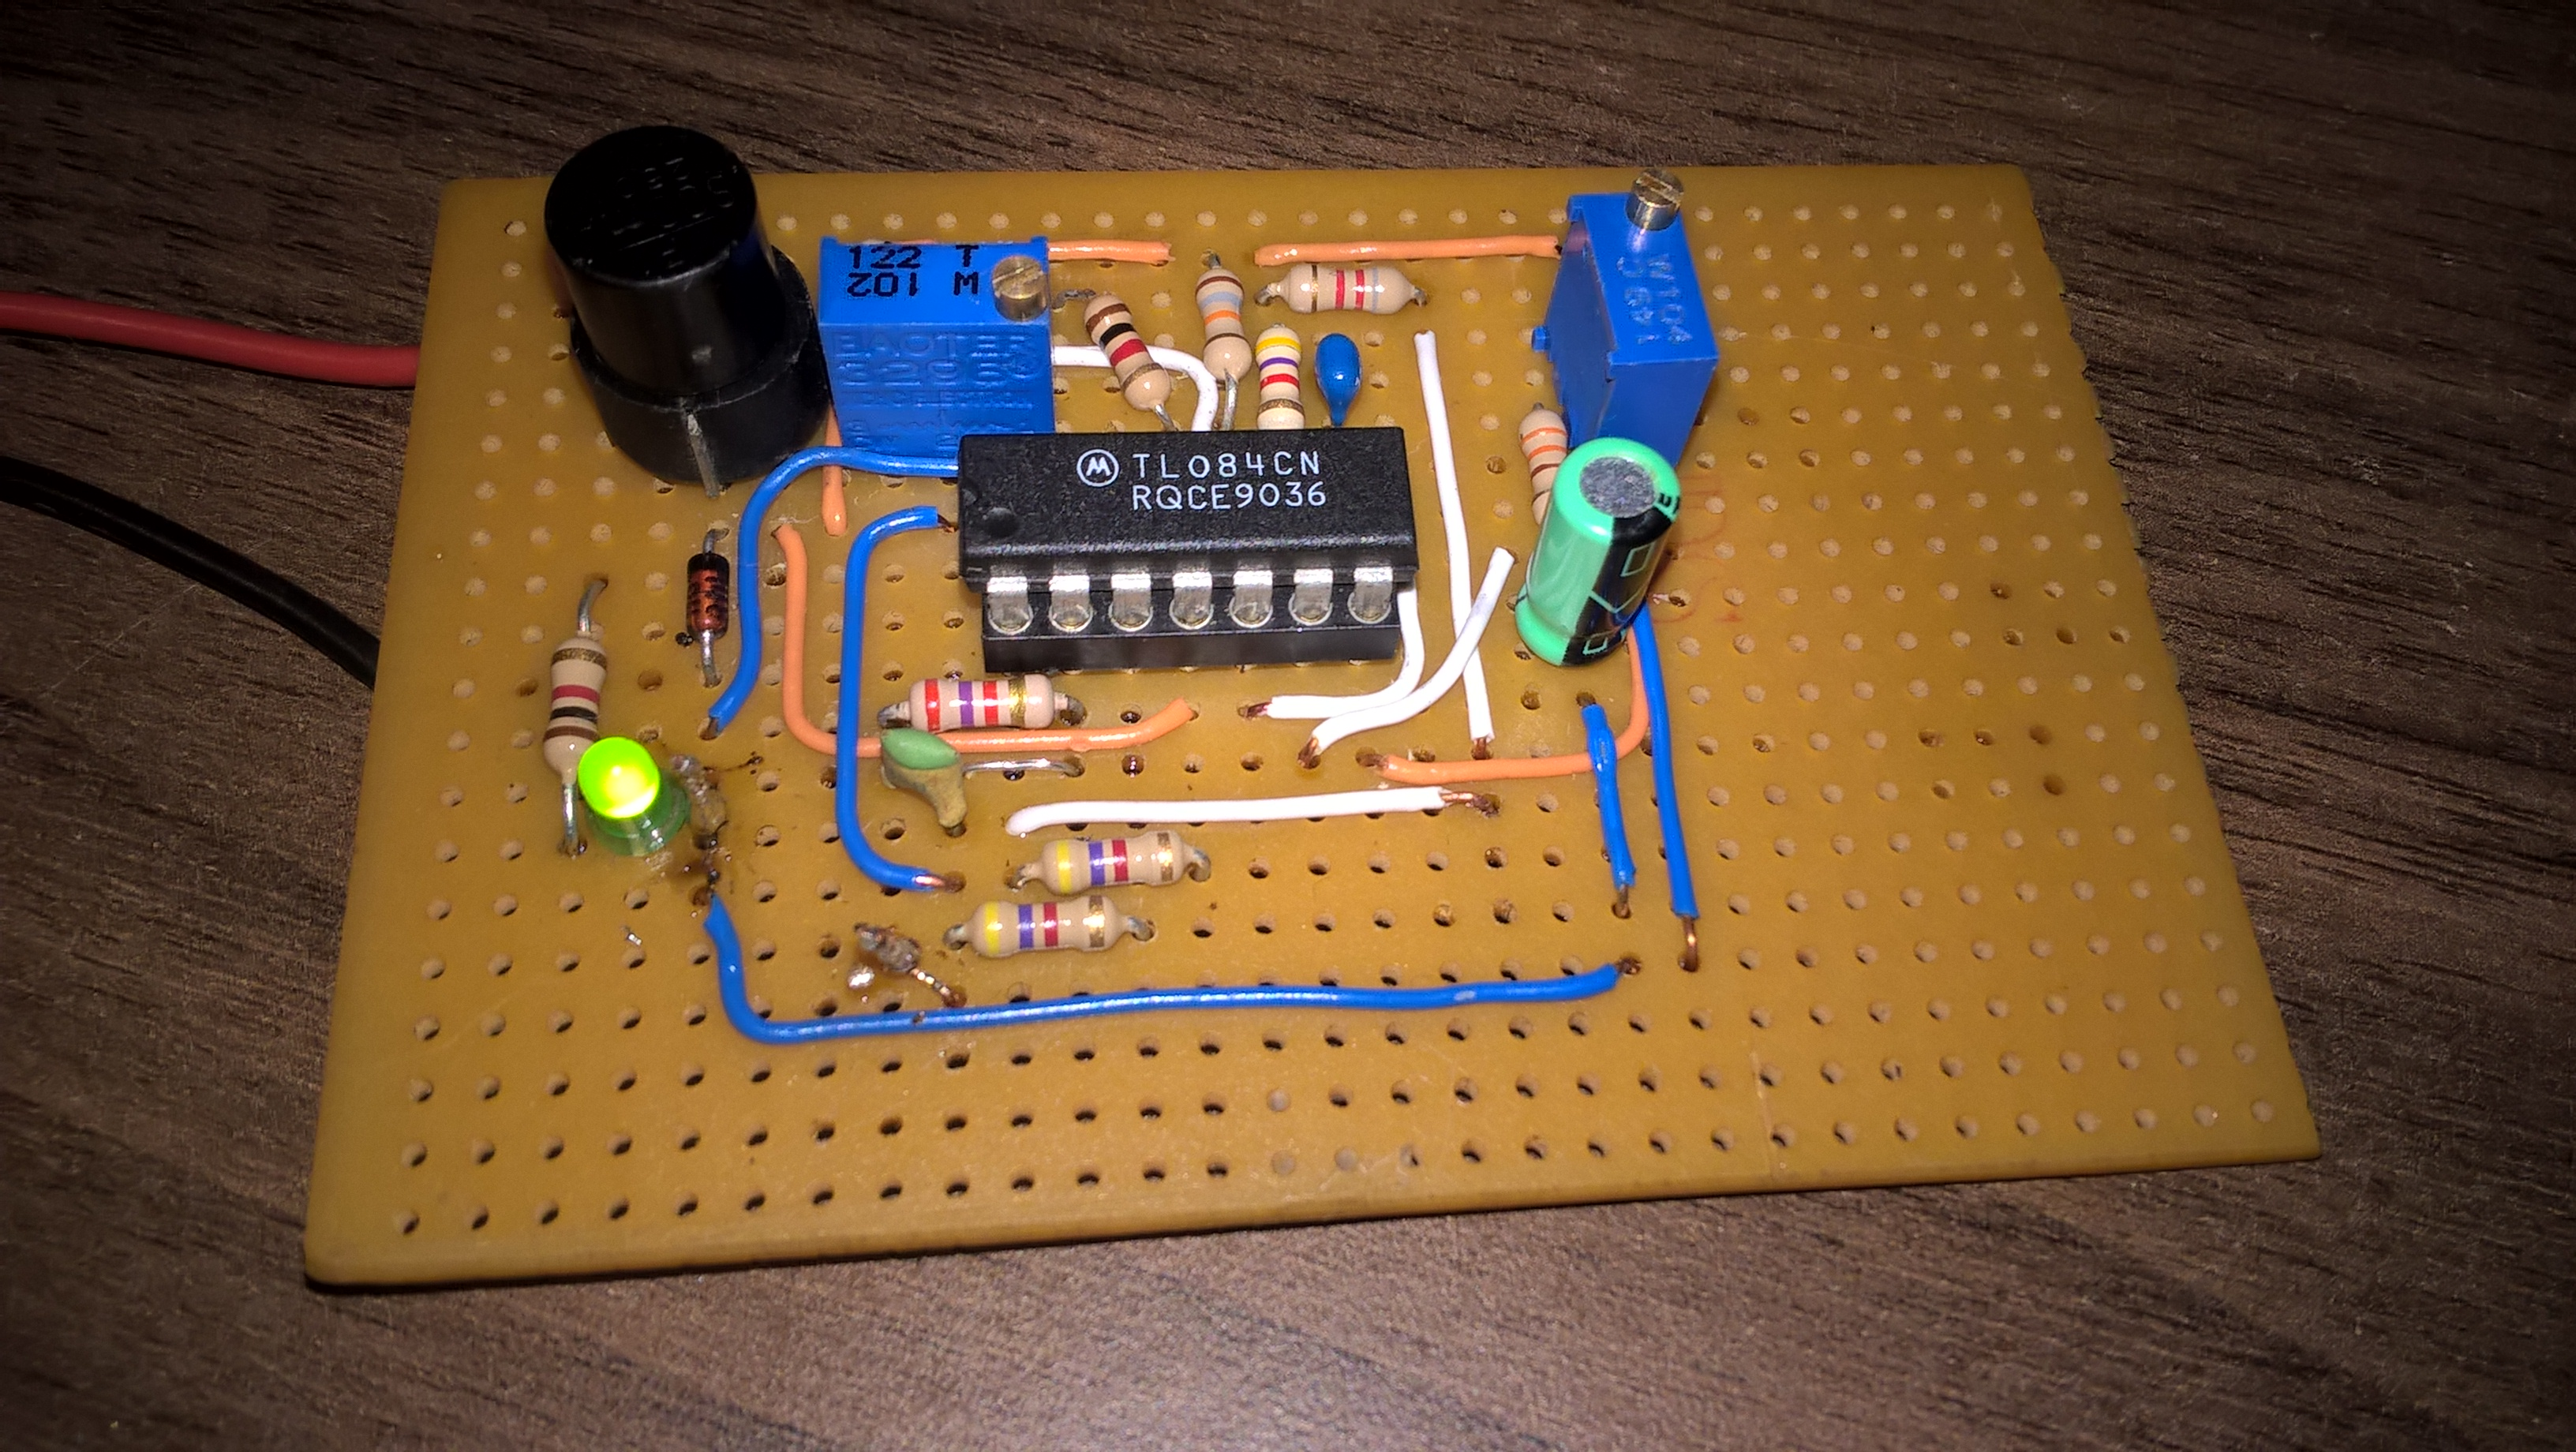
\includegraphics[scale=0.15]{./image/placa_1.jpg}\\
	\caption{Top View}
\end{figure}
\begin{figure}[H]
	\centering
	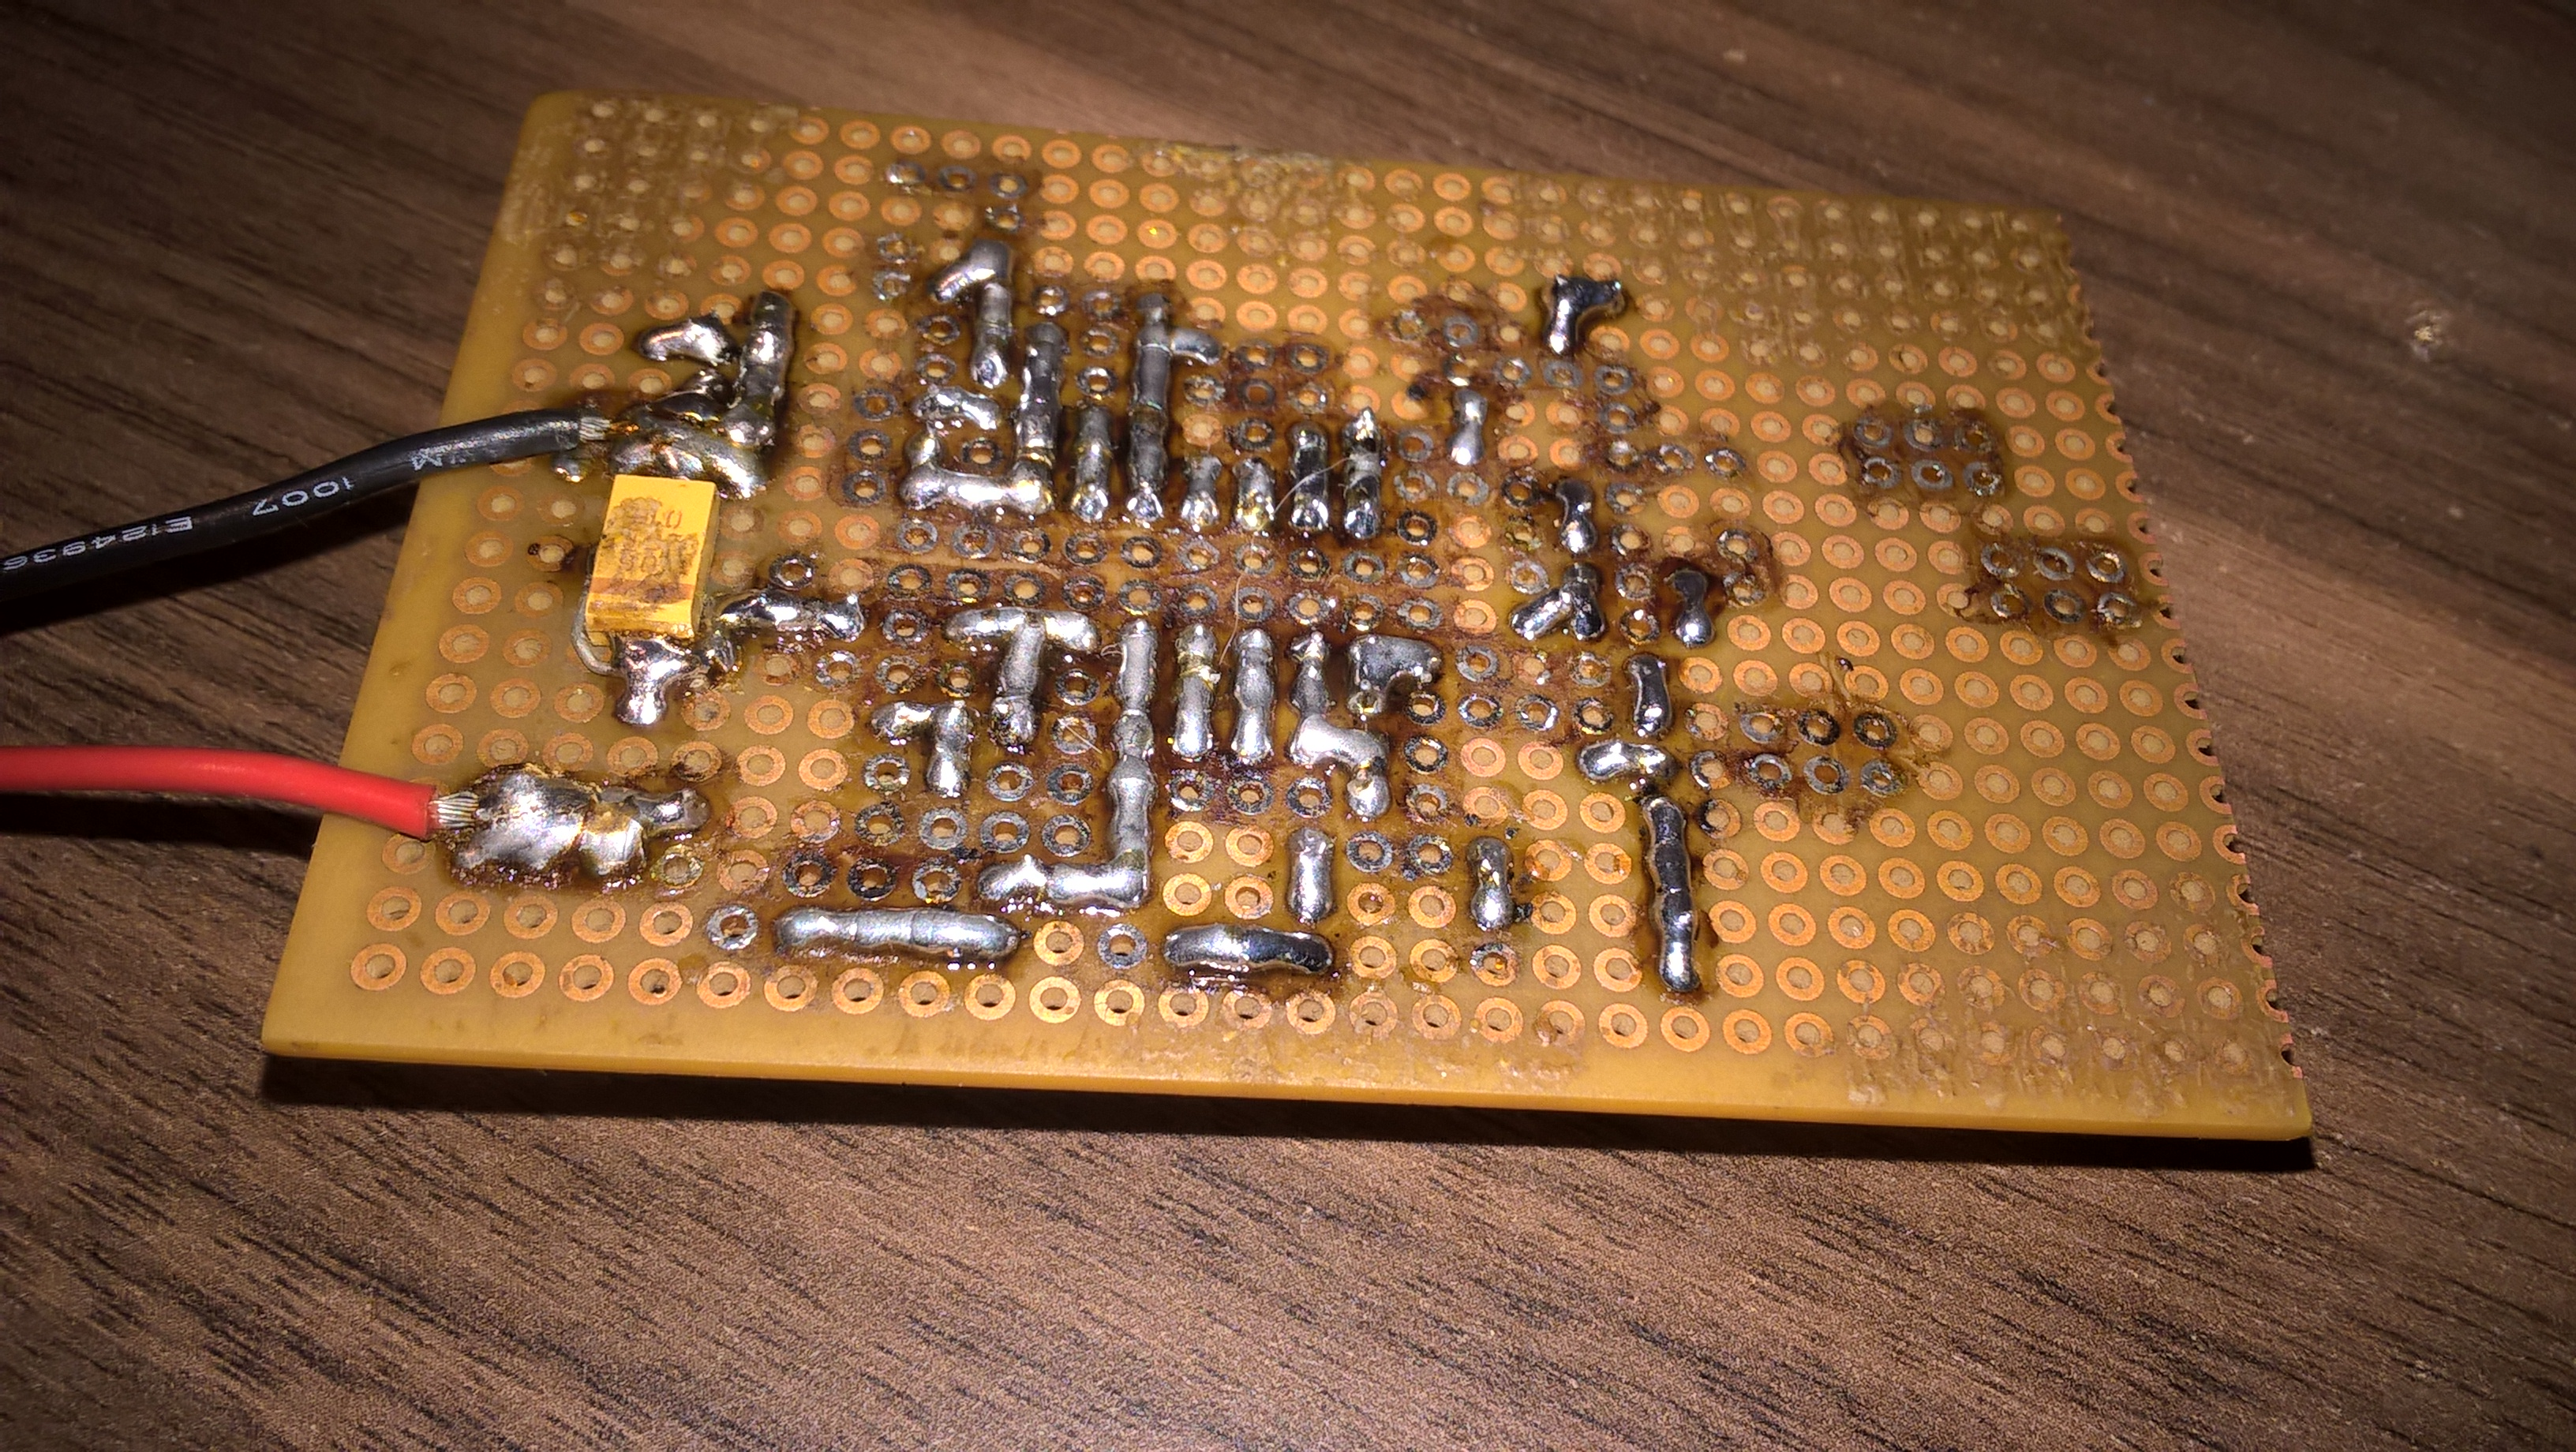
\includegraphics[scale=0.15]{./image/placa_2.jpg}\\
	\caption{Back View}
\end{figure}\par
%%%%%%%%%%%%%%%%%%%%%%%%%%%%%%%%%%%%%%%%%%%%%%%%%%%%%%%%%%%%%%%%%%%%%%%%%%%
\section{Simulação}
%\begin{comment}	
\begin{figure}[H]
	\centering
	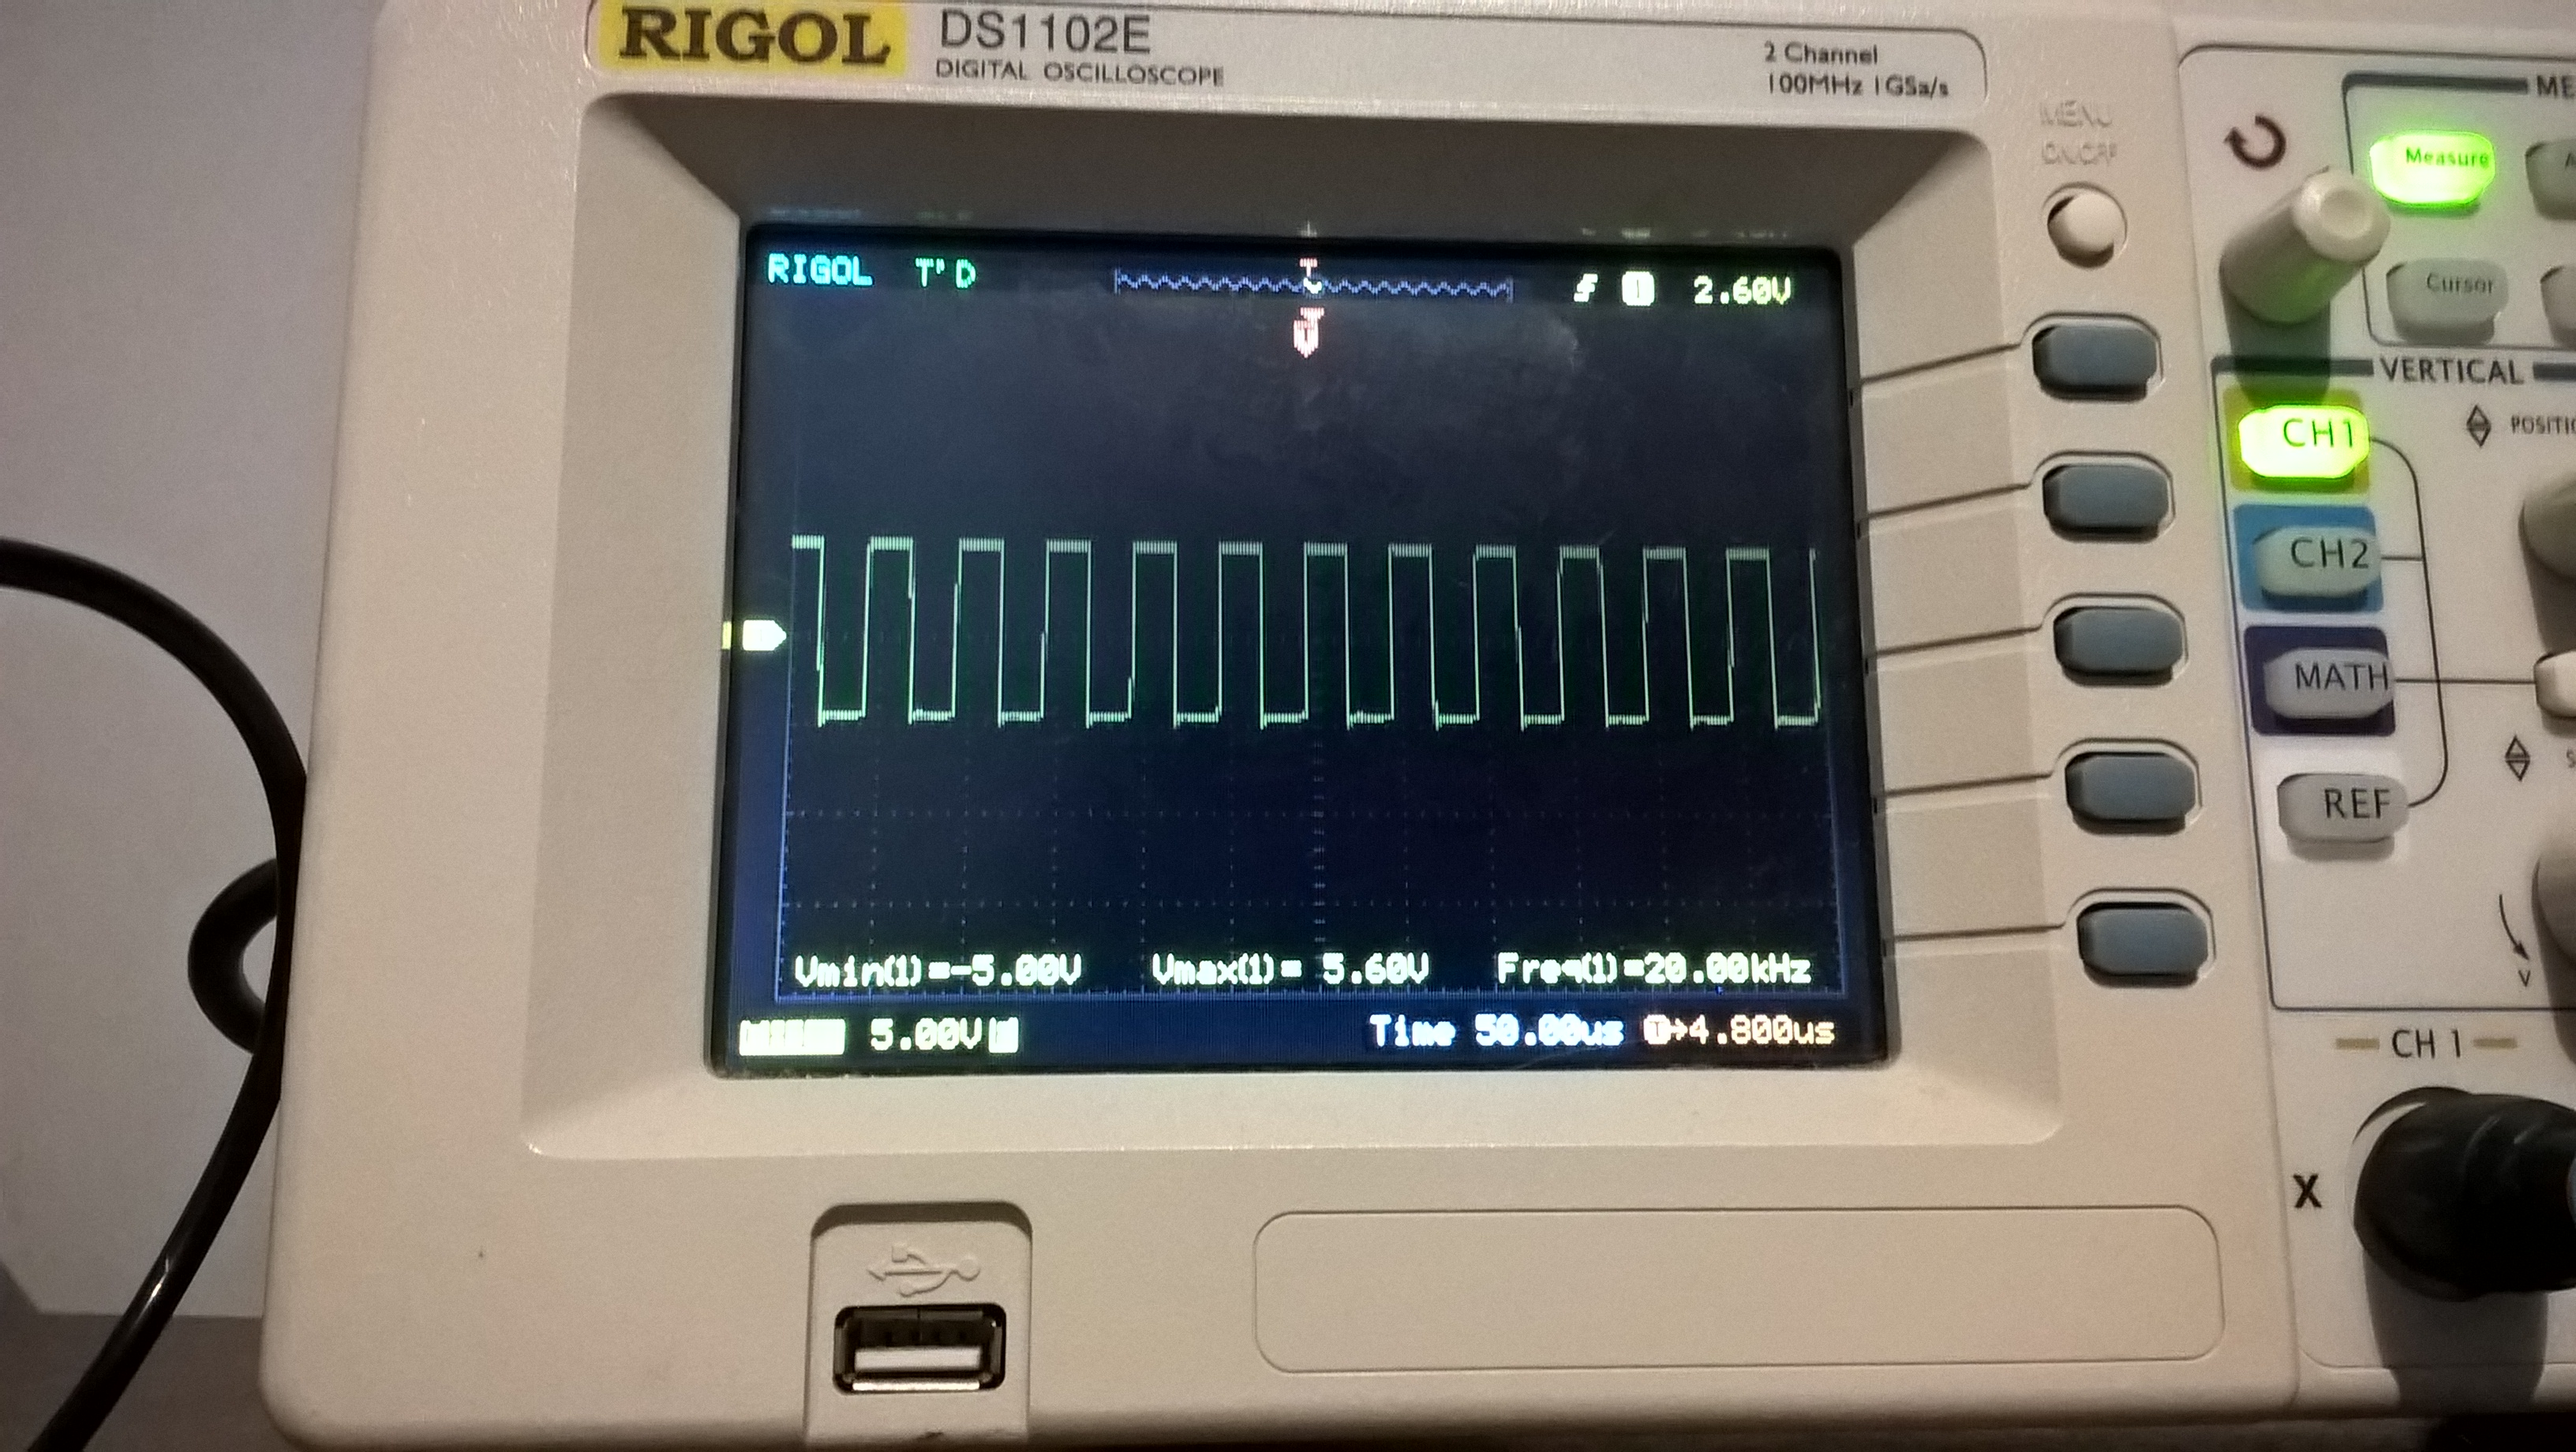
\includegraphics[scale=0.15]{./image/quadrado.jpg}\\
	\caption{Onda Quadrada}
\end{figure}
\begin{figure}[H]
	\centering
	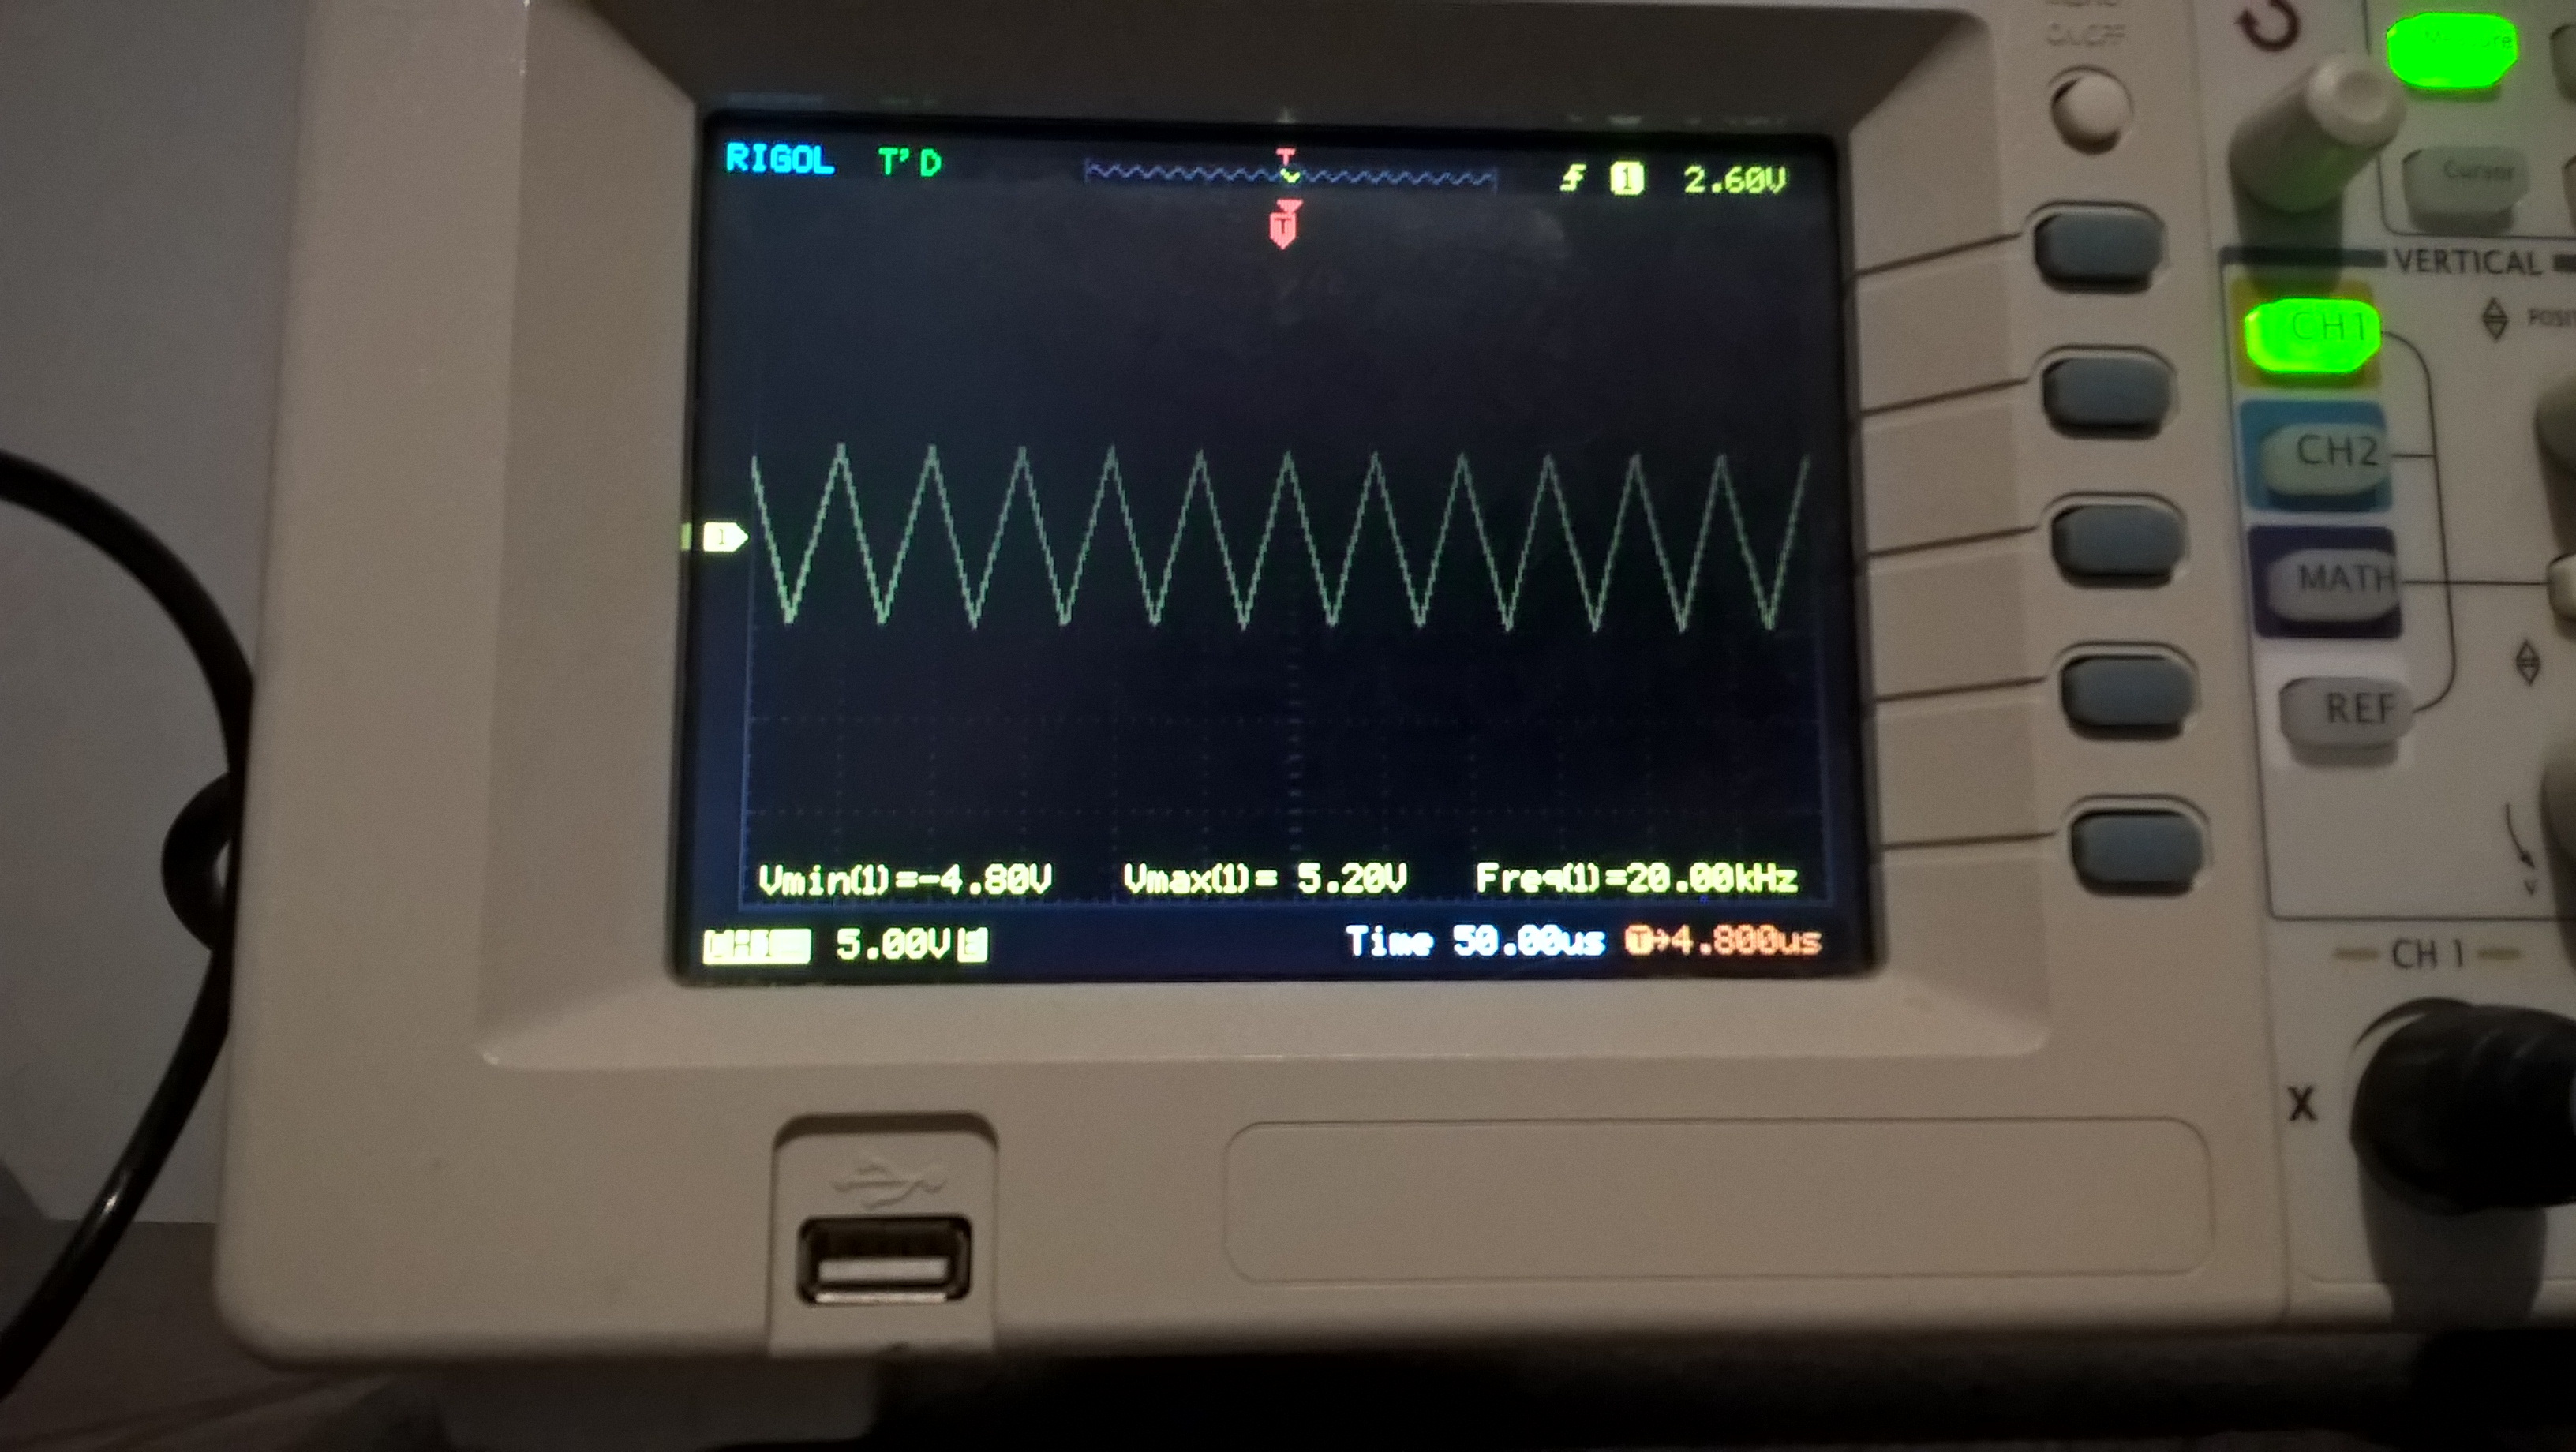
\includegraphics[scale=0.15]{./image/triangulo.jpg}\\
	\caption{Onda Triangular}
\end{figure}\par
\newpage
%%%%%%%%%%%%%%%%%%%%%%%%%%%%%%%%%%%%%%%%%%%%%%%%%%%%%%%%%%%%%%%%%%%%%%%%%%%
\newpage
\footnote{Apontamentos}
%
	\end{document}
%%%%%%%%%%%%%%%%%%%%%%%%%%%%%%%%%EOF%%%%%%%%%%%%%%%%%%%%%%%%%%%%%%%%%%%%%%%
